\documentclass[12pt,a4paper]{article}

\usepackage{style2017}
\usepackage{hyperref}

\hypersetup{
    colorlinks =false,
    linkcolor=blue,
   linkbordercolor = 1 0 0
}
\newcounter{numexo}
\setcellgapes{1pt}

\begin{document}


\begin{NSI}
{TP}{Langage machine}
\end{NSI}



Il existe sur le web un simulateur pour réaliser des instructions en langage assembleur/machine à l'adresse : \textsf{https://www.peterhigginson.co.uk/AQA/}\medskip

\begin{center}
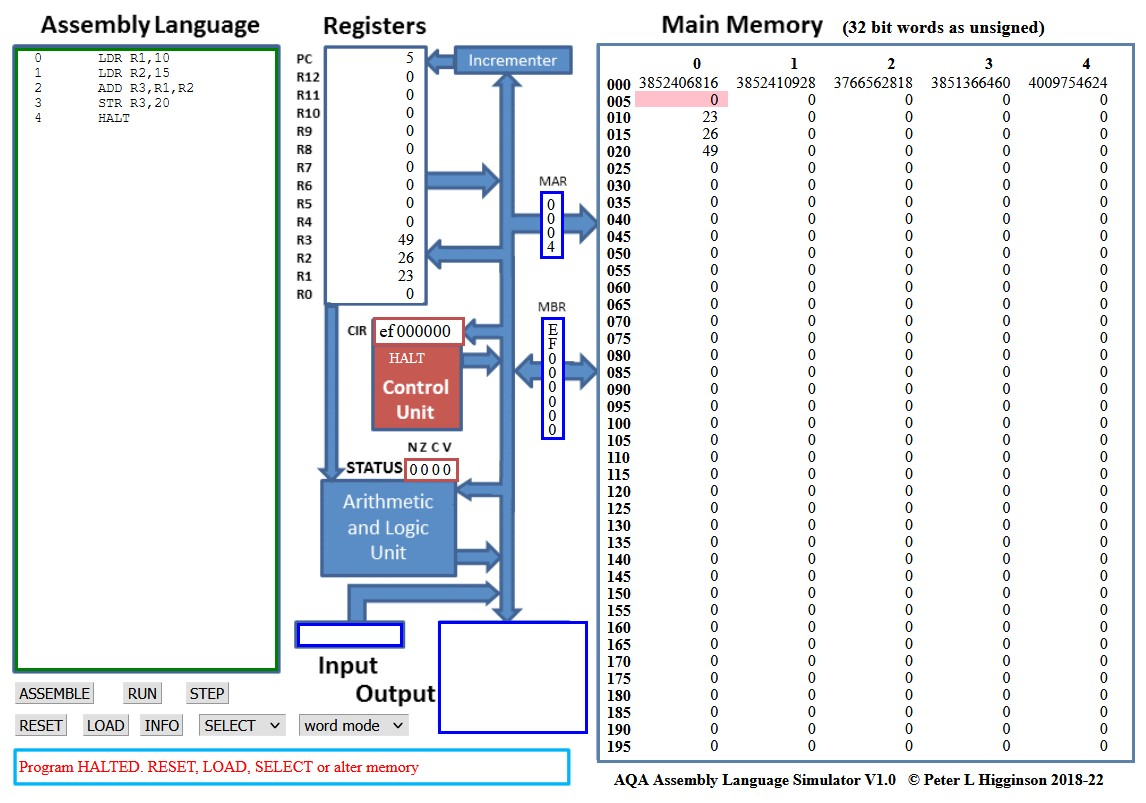
\includegraphics[scale=0.8]{../img/simulateur.jpg}
\end{center}

On donne ci-dessous les \textbf{principales instructions} du langage assembleur:\medskip

L'opérande <opérande> est une valeur désignée par \textsf{\#n}  ou \textsf{Rm} pour utiliser le contenu du registre Rm. 

\begin{itemize}
\item \textsf{LDR Rd, <mem ref>} : Charge la valeur stockée dans l'emplacement mémoire spécifié par <mem ref> dans le registre d.\medskip
\item \textsf{STR Rd, <mem ref>} : Stocke la valeur du registre d dans l'emplacement mémoire spécifié par <mem ref>.\medskip
\item \textsf{ADD Rd, Rn, <opérande>} : Ajoute la valeur spécifiée dans <opérande> à la valeur dans le registre n et stocke le résultat dans le registre d.\medskip
\item \textsf{SUB Rd, Rn, <opérande>} :  Soustrait la valeur spécifiée par <opérande> de la valeur dans le registre n et stocke le résultat dans le registre d.\medskip 
\item \textsf{MOV Rd, <opérande>} : Copie la valeur spécifiée par <opérande> dans le registre d.\medskip
\item \textsf{CMP Rn, <opérande>} : Compare la valeur stockée dans le registre n avec la valeur spécifiée par <opérande>.\medskip
\item \textsf{B <label>} : Branche toujours sur l'instruction à la position <label> dans le programme.\medskip
\item \textsf{B <condition> <label>} : Branche conditionnellement à l'instruction à la position <label> dans le programme si la dernière comparaison répond aux critères spécifiés par la <condition>. 
Les valeurs possibles pour <condition> et leur signification sont : EQ pour Égal à, NE pour Non égal à, GT pour Supérieur à et LT pour Inférieur à.\medskip
\item \textsf{AND Rd, Rn, <opérande>} :  Effectue une opération ET logique au niveau du bit entre la valeur dans le registre n et la valeur spécifiée par <opérande> et stocke le résultat dans le registre d.\medskip
\item \textsf{ORR Rd, Rn, <opérande>} :  Effectue une opération OU logique au niveau du bit entre la valeur dans le registre n et la valeur spécifiée par <opérande> et stocke le résultat dans le registre d.\medskip
\item \textsf{EOR Rd, Rn, <opérande>} :  Effectue une opération logique binaire ou exclusif (XOR) entre la valeur dans le registre n et la valeur spécifiée par <opérande> et stocke le résultat dans le registre d.\medskip
\item \textsf{MVN Rd, <opérande>} : Effectue une opération NON logique au niveau du bit sur la valeur spécifiée par <opérande> et stocke le résultat dans le registre d.\medskip
\item \textsf{LSL Rd, Rn, <opérande>} : Décale logiquement à gauche la valeur stockée dans le registre n du nombre de bits spécifié par <opérande> et stocke le résultat dans le registre d.\medskip
\item \textsf{LSR Rd, Rn, <opérande>} : Décale logiquement à droite la valeur stockée dans le registre n du nombre de bits spécifié par <opérande> et stocke le résultat dans le registre d.\medskip
\item \textsf{HALT} : Arrête l'exécution du programme. 
\end{itemize}
    
\section*{Langages}

\begin{enumerate}
\item Qu'est-ce que le langage machine ? \vspace{3cm}
\item Qu'est-ce que le langage assembleur ? \vspace{3cm}
\item Comment un programme écrit en langage de haut niveau est-il transformer en langage machine ?\vspace{3cm}
\end{enumerate}


\section*{Langage assembleur}

\begin{enumerate}
\item Décrire par des phrases ce que font les différentes instructions suivantes écrites en langage assembleur.\medskip
\begin{enumerate}

\item ADD R0, R1, \#25 \vspace{1.5cm}
\item LDR R2,64 \vspace{1.5cm}
\item MOV R3, \#45 \vspace{1.5cm}
\item STR R4, 72 \vspace{1.5cm}
\item SUB R5,R2,R3 \vspace{1.5cm}
\item CMP R3, \#25 \\
\hspace{0.5cm}BGT 15 \vspace{1.5cm}
\end{enumerate}

\item Sur la capture de la première page, un programme en langage assembleur est donné. Que réalise ce programme ? \vspace{2cm}

\item Écrire en langage assembleur correspondant les instructions décrites par les phrases suivantes:
\begin{itemize}
\item Place la valeur 15 dans le registre R0 \vspace{1cm}
\item Place la valeur 7 dans le registre R1 \vspace{1cm}
\item Additionne la valeur stockée dans le registre R0 et la valeur stockée dans le registre R1, le résultat est stocké dans le registre R5 \vspace{1cm}
\item Place le contenu du registre R5 à l'adresse mémoire 125. \vspace{1cm}
\item Place la valeur 10 dans le registre R1 \vspace{1cm}
\item Place la valeur stockée à l'adresse mémoire 125 dans le registre R0 \vspace{1cm}
\item Soustrait la valeur stockée dans le registre R0 et la valeur stockée dans le registre R1, le résultat est stocké dans le registre R5 \vspace{1cm}
\item Place le contenu du registre R5 à l'adresse mémoire 125. \vspace{1cm}
\end{itemize}
\item Quelles sont les valeurs dans les différents registres à l'issu de ce programme ? \vspace{2cm}
\item Saisir votre programme dans le simulateur et vérifier vos réponses.
\end{enumerate}



\end{document}

